%
\chapter{Opazovanje vesoljskega vremena }
\label{Vaje:VesVrem} % Always give a unique label
% use \chaptermark{}
% to alter or adjust the chapter heading in the running head

Ugotovite smisel poznavanja vesoljskega vremena, značilnosti pojavov, pripravite poskus in vesoljsko vreme spremljajte vsaj dva tedna.

\section{Pomen naloge}
\label{sec:VesVremPomen}
 Vsakdo ve, da ima Sonce največji vpliv na pojave v okolici zemeljske atmosfere. Bralec, ki samo preleti študentsko poročilo \cite{VesVreme_2014}, si že uredi prvi vtis o vesoljskem vremenu (angl.\textit{ space weather}). Učinke pojavov v vesolju čutijo načrtovalci in uporabniki radijskih zvez, satelitske navigacije in celo sistemov za prenos električne energije. Napovedovanje sprememb vesoljskega vremena in njihovih učinkov, tudi v praksi bodočega pomorščaka, temelji na skrbnem beleženju podatkov opažanj in njihovem obdelovanju.   

\section{Vloge v skupini}
\label{sec:VesVrem_Vloge}
Skupino sestavljate vsaj štirje člani, ki si med seboj tudi pomagate, vendar vsak nosi odgovornost za svoj del.

\begin{table}
	\centering
	\caption{Oris vlog skupine Opazovanje vesoljskega vremena}
	\label{tab:VesVremVloge} 
	\begin{tabular}{c|c|l}
		\hline\noalign{\bigskip}
		število & odgovornost & rezultat dela \\
		\noalign{\smallskip}\hline\noalign{\smallskip}
		1 & iskalec literature & izvleček najdenega\\
		1 & zapisovalec stanj, napovedi & pregled uresničitev napovedi \\
		1 & priprava in izvedba poskusa & razumevanje poskusa \\
		1 & predstavitev & izvleček izvirnega dela skupine \\ \hline
		vsi & poročilo & poglobitev razumevanja vesoljskega vremena\\
		\noalign{\smallskip}\hline
	\end{tabular}
\end{table}

\subsection{V pregledu literature se osredotočite in zapišite izvleček}
\label{subsec:VesVrem_ZapIzvlLit}

\textbf{Nasvet} Bodite praktični. Razmislite kaj boste napisali v izvlečku, predvsem pa najdite odgovor na vprašanje, ki si ga boste kot skupna zastavili v začetku. Na primer: \textit{Kaj podatki o vesoljskem vremenu lahko pomagajo pomorščaku med plovbo po Sredozemlju? Kako jih lahko pridobi in kako upošteva?}

Predvsem z dejstvi in razlagami nadgradite dosedanje študentske zapise. Izberite tiste, ki vam kot navdušenemu spoznavalcu najbolj nazorno povedo katere pojave na Soncu znastveniki sploh spremljajo, s katerimi veličinami jih opisujejo in seveda kako spremembe teh veličin vplivajo na razmere v atmosferi.

Primer zanimive veličine je število vseh prostih elektronov (angl. Total Electron Content, TEC) v atmosferski plasti, ki jo imenujemo ionosfera. TEC je posebno zanimiv podatek za navigatorjev satelitski navigacijski sprejemnik. Znanstveniki prostor ionosfere zaradi praktičnosti razdelijo na kockam podobne segmente in za vsakega posebej izmerijo oz. ocenijo TEC. Za ocenjevanje učinkov na navigacijski sprejemnik je pomembno le število prostih elektronov, ki jih elektromagnetni val s satelita sreča v \textit{navidezni, zaradi loma ukrivljeni, cevi} do posameznega sprejemnika.
      
Od slovenskih virov priporočamo, da si najprej ogledate \href{http://www.s50e.si/multimedija}{\textit{video Nastanek in vplivi Sončevih aktivnosti}}, za razlago učinkov na navigacijske sprejemnike pa si preberite članka  \href{http://www.ltfe.org/wp-content/uploads/2011/09/sternobcutljivost_sprejemnikovp.pdf}{\textit{Občutljivost sprejemnikov GPS na Sončeve radijske izbruhe}} ter \href{http://www.fgg.uni-lj.si/sugg/referati/2013/SZGG_2012_Berk_Bajec_Radovan.pdf}{\textit{Spremljanje ionosferskih motenj nad Slovenijo s pomočjo omrežja stalnih GNSS-postaj SIGNAL}}. Izredno podroben in z opazovanji podprt gimnazijski pogled na dogajanje na površini Sonca dobro povzema \href{http://www2.arnes.si/~gljsentvid10/Opazovanje_Sonceve_povrsinske_aktivnosti.pdf}{\textit{seminarska naloga}}.

Mednarodne lestvice \textit{nevihtnih pojavov} RSG (angl. Radio blackouts, Solar radiation storms, Geomagnetic storms) boste našli na \href{http://www.swpc.noaa.gov/noaa-scales-explanation}{\textit{naslovu NOAA}}. Na istem strežniku najdete trenutne obete sprememb vesoljskega vremena: za \href{http://www.swpc.noaa.gov/communities/radio-communications}{\textit{radijske zveze}}, za \href{http://www.swpc.noaa.gov/communities/global-positioning-system-gps-community-dashboard}{\textit{satelitsko navigacijo}} in za  \href{http://www.swpc.noaa.gov/communities/electric-power-community-dashboard}{\textit{električna omrežja}}.

%Andrej Štern (diapozitivi) 
%\verb|http://www.s50e.si/wp-content/uploads/2012/10/S50E-55LET-S57BAJ.pdf|

%Marko Munih: Prednosti SDR tehnologije na KV in UKV
 
Za bolj zahtevne bralce priporočamo pregled revije \href{http://agupubs.onlinelibrary.wiley.com/agu/journal/10.1002/(ISSN)1542-7390/}{\textit{Space Weather}}.

\subsection{Sestavite kritičen pregled trenutnih vrednosti in napovedi}
\label{subsec:VesVrem_Podat}
Trenutne bistvene podatke o sončnem ciklusu najdete na \href{http://www.swpc.noaa.gov/SolarCycle/}{\textit{strani s podatki o številu sončnih peg ...}} ali \href{http://www.swpc.noaa.gov/products/solar-cycle-progression}{stran s pregledom zadnjih dveh ciklusov Sončeve dejavnosti (pege, pretok z valovno dolžino 10,7 cm in $A_p$ planetarni indeks)}. Od podatkovnih baz priporočamo pregled  \href{http://www.spaceweather.org/}{\textit{mednarodnega spletišča}}, odkoder lahko vstopite v centre za opazovanje vesoljskega vremena s celega sveta, v katerih objavljajo podatke opazovanj ionosfere, trenutne hitrosti in pretoka Sončevega vetra, izmerjene vrednosti lokalnega magnetnega polja Zemlje na posameznem območju. Nekateri centri podajajo tudi podatke za vso Zemljo, še posebno podatek o planetarnem indeksu $K_p$, za katerega ugotovite, kaj sploh pomeni.

Evropsko spletišče ESWP zbira na strani podatke iz območnih evropskih centrov IAP Češka, LSWC Švedska, SIDC Belgija) in SRC Poljska, kjer poleg stanja sproti objavlja tudi  \href{http://www.spaceweather.eu/sl/nowforecasting}{\textit{trenutne napovedi}}, vsak mesec pa objavljajo \href{http://www.stce.be/newsletter/pdf/2015/STCEnews20151002.pdf}{takšna poročila}. Znotraj ameriške agencije NOAA deluje SWPC, ki ponuja \href{http://www.swpc.noaa.gov/sites/default/files/images/u33/primer_2010_new.pdf}{\textit{razlago osnovnih značilnosti vesoljskega vremena}}. V SWPC so  \href{http://www.swpc.noaa.gov/communities/space-weather-enthusiasts}{\textit{za zanesenjake sestavili stran}}, ponujajo pa tudi \href{http://www.swpc.noaa.gov/products/aurora-3-day-forecast}{\textit{tridnevne napovedi polarnih sijev}}. Ruska IAG tudi objavlja svoje \href{http://www.tesis.lebedev.ru/en/forecast_activity.html}{\textit{trenutne napovedi}}. Avstralski IPS prinaša  \href{www.ips.gov.au}{\textit{pojmovnik vesoljskega vremena}} in \href{http://www.ips.gov.au/Satellite/2/2}{\textit{stanje TEC}}. Japonski NICT posebej spremlja \href{http://wdc.nict.go.jp/IONO/index_E.html}{\textit{razširjanje radijskih valov v trenutnih pogojih}} vesoljskega vremena.


\begin{figure}
	\centering
	% Use the relevant command for your figure-insertion program
	% to insert the figure file.
	% For example, with the option graphics use
	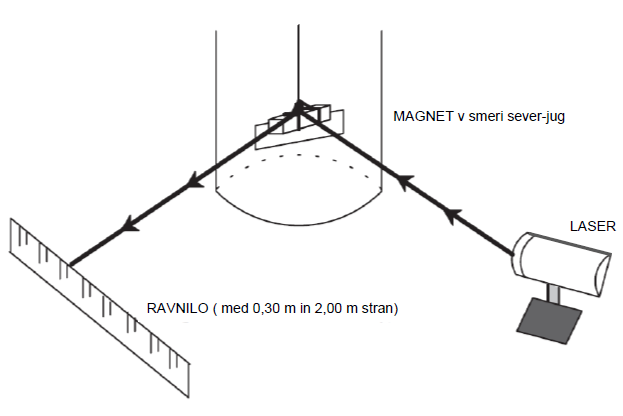
\includegraphics[height=6cm]{Vaje/VesoljVreme/figs/Eksp.png}
	%
	% If not, use
	%\picplace{5cm}{2cm} % Give the correct figure height and width in cm
	%
	\caption{Tako izgleda domači magnetometer v marmeladnem loncu. Prirejeno po: \textit{Solar Physics and terrestrial effects, NOAA}}
	\label{fig:VesVr_Eksp}       % Give a unique label
\end{figure}
 
\subsection{Potrdite vpliv Sončevega vetra na magnetno polje Zemlje z vašo opazovalnico}
\label{subsec:VesVrem_Posk}
Kako pripravite magnetometer v loncu za marmelado na sliki \ref{fig:VesVr_Eksp} in lahko z njim izvedete poskus, je natančno opisano v \href{http://www.swpc.noaa.gov/sites/default/files/images/u33/Activity_7.pdf}{\textit{Solar Physics and terrestrial effects Activity 7: The Effect of the Solar Wind on the Geomagnetic Field}}. Sami boste torej poskusno spremljali spremembe v vodoravni komponenti lokalnega magnetnega polja Zemlje. Če natančni pri izdelavi, če boste dovolj dobro izbrali prostor, natančno postavili napravo, skrbno opazovali odklon ter se boste povezali s sodelavcem, ki sestavlja pregled napovedi v \ref{subsec:VesVrem_Podat}, boste v časih napovedanih sprememb bolj pogosto (na 10 minut) beležili usmerjenost magneta in tako morda potrdili spremembe vesoljskega vremena. Med časom natančnejšega opazovanja vključite tudi magnetometer, ki ga vsebuje večsenzorska škatlica MTi.


\subsection{Oprema}
\label{subsec:VesVrem_Oprema}
Večina vas bo potrebovala le računalnik, priključen na medomrežje. Za poskus pa boste potrebovali še nekaj dodatnih pripomočkov, ki jih čimprej pripravite. Preskrbite si magnetometer v škatlici MTi in se ga naučite uporabljati.

%\section{Spletnjača}
%\label{sec:VesVrem_Splet}

%Pregled virov, ki so našteti med opisi nalog članov skupine.

%(1)   \url{http://www.s50e.si/multimedija}\\[2mm]
%(2)   \verb|.. /2011/09/sternobcutljivost_sprejemnikovp.pdf| \\
%(3)   \verb|.. /sugg/referati/2013/SZGG_2012_Berk_Bajec_Radovan.pdf| \\
%(4)   \verb|.. /Opazovanje_Sonceve_povrsinske_aktivnosti.pdf| \\
%(5)   \url{http://www.swpc.noaa.gov/noaa-scales-explanation}\\[2mm]   
%(6)   \url{http://www.swpc.noaa.gov/communities/radio-communications}\\[2mm]   
%(7)   \verb|.. /global-positioning-system-gps-community-dashboard| \\   
%(8)   \verb|... /communities/electric-power-community-dashboard|  \\ 
%(9)   \verb|..wiley.com/agu/journal/10.1002/(ISSN)1542-7390/ |  \\   
%(10)  \url{http://www.swpc.noaa.gov/products/solar-cycle-progression}\\[2mm]   
%(11)  \url{http://www.spaceweather.org/}\\[2mm]   
%(12)  \url{http://www.spaceweather.eu/sl/nowforecasting}\\[2mm]   
%(13)  \verb|.. /sites/default/files/images/u33/primer_2010_new.pdf|  \\   
%(14)  \url{http://www.swpc.noaa.gov/communities/space-weather-enthusiasts}\\[2mm]  
%(15)  \url{http://www.swpc.noaa.gov/products/aurora-3-day-forecast}\\[2mm]   
%(16)  \url{http://www.tesis.lebedev.ru/en/forecast_activity.html}\\[2mm]   
%(17)  \url{www.ips.gov.au}\\[2mm]   
%(18)  \url{http://www.ips.gov.au/Satellite/2/2}\\[2mm]   
%(19)  \url{http://wdc.nict.go.jp/IONO/index_E.html}\\[2mm]   
%(20)  \verb|.. noaa.gov/sites/default/files/images/u33/Activity_7.pdf|

\subsection{Dostopi}
Dostop do naslovov spletnih dokumentov najdete na strani \url{www.forumgnsss.si}, kjer v rubriki \textit{Za študente} izberite \textit{spletnjača vesoljsko vreme}.


%
% For built-in environments use
%
% Problems or Exercises should be sorted chapterwise
\section*{Povzetek nalog}
\addcontentsline{toc}{section}{Problems}
%
% Use the following environment.
% Don't forget to label each problem;
% the label is needed for the solutions' environment
\begin{prob}
\label{Nal:VesVrem_Izvl}
\textbf{Izvleček naj bo uvod v poročilo}\\
(a) V skupini si zastavite največ tri praktična vprašanja v zvezi z vesoljskim vremenom. \ref{subsec:VesVrem_ZapIzvlLit} \\
(b) Zapišite izvleček izbora besedil, s katerim si boste na vprašanja odgovorili.
\end{prob}

\begin{prob}
\label{Nal:VesVrem_Belez}
\textbf{Beležite podatke o vplivih Sončevega vetra}\\
(a) Izberite katere podatke o stanju in napovedih boste beležili. \ref{subsec:VesVrem_Podat}\\
(b) Beležite vsaj 15 dni. \\
(c) V poročilu kritično zapišite ujemanja med napovedmi in dejanskimi pojavi.
\end{prob}

\begin{prob}
	\label{Nal:VesVrem_Eksp}
	\textbf{Opazujte vpliv Sončevega vetra na magnetno polje Zemlje}\\
	(a) Sestavite napravo za opazovanje.\ref{subsec:VesVrem_Posk} \\
	(b) Izvedite poskus. \\
	(c) Posvetujte se z ostalimi člani in napišite poročilo o svojih opažanjih.
\end{prob}


\begin{prob}
\label{Nal:VesVrem_Predst}
\textbf{Predstavite opravljeno delo celotne skupine}\\
(a) Pomagajte ostalim članom pri njihovem delu. \\
(b) Poskrbite, da je skupina v \textbf{rednem} stiku s predavatelji.\\
(b) Spremljajte napredek in sestavite osnutek poročila. \\
(č) Po oddanem poročilu pripravite 5 minutno predstavitev na tabli.
\end{prob}

%
